\chapter{Entorno Empresarial}
\label{capitulo1}
\lhead{Capítulo 1. \emph{Entorno Empresarial}}

En este capítulo se explica el entorno laboral en el cual el
estudiante desenvolvió su proyecto de pasantía. Se da una descripción
de la empresa Everis, con su visión y valores, y se muestra
como se encuentra organizada la empresa.


\section{Everis}

Everis es una empresa multinacional que se dedica a la consultoría y
\emph{outsourcing} abarcando todos los sectores del ámbito económico.
Actualmente Everis cuenta con alrededor de 19.000
empleados repartidos entre USA, Europa y Latinoamérica.

Desde el año 2014 Everis se unió al grupo NTT DATA, la sexta empresa de
servicios IT del mundo, con 100.000 profesionales y presencia en Asia-Pacífico,
Oriente Medio, Europa, Latinoamérica y Norteamérica.

Pero por encima de todo en Everis se cree en las personas, en su desarrollo integral y en
el talento que representan. En everis apuestan firmemente por el talento, y
su principal objetivo es conseguir un alto rendimiento profesional al crear
un contexto de libertad responsable (\cite{EVERIS}).

\subsection{Visión}

''Everis es una compañía de ámbito mundial, excepcional en términos éticos y
emocionales, liderada por valores y donde cualquier sueño es alcanzable.'' (\cite{EVERIS}).

\subsection{Valores}

\begin{itemize}
  \item \textbf{Generosidad exigente}: compartimos para hacer.
  \item \textbf{Libertad responsable}: hacemos lo que queremos.
  \item \textbf{Energía creativa}: nos apasiona lo que hacemos.
  \item \textbf{Coherencia}: hacemos lo que decimos.
  \item \textbf{Transparencia}: contamos lo que hacemos. (\cite{EVERIS})
\end{itemize}

\subsection{Organización de la empresa}

Everis España está dividida en líneas operativas y por sectores
dependiendo del tipo de servicio/proyecto o conocimientos que se requieren (\cite{MANUAL}).

Las unidades operativas de Everis España se muestran en la figura \ref{unidades}.
El pasante formaba parte de la unidad operativa de Tecnología.

\begin{figure}[h!]
\centering
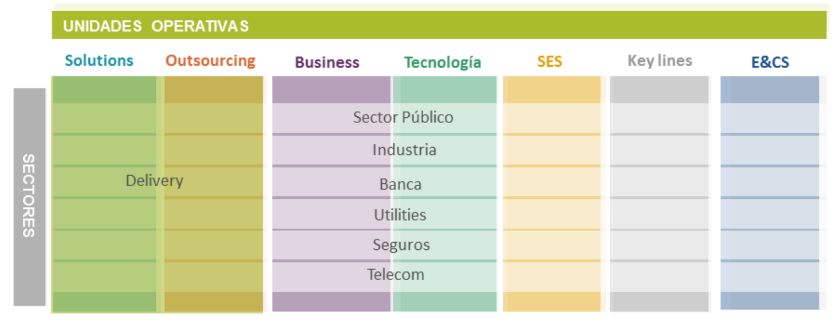
\includegraphics[width=\textwidth]{UnidadesOperativas}
\caption[Unidades Operativas de Everis]{Unidades operativas en las que
        está dividida Everis España (\cite{MANUAL}).}
\label{unidades}
\end{figure}


Luego, dentro de cada unidad operativa los consultores se diferencian por categorías.
Las categorías presentes en la unidad operativa de Tecnología se muestran en la
figura \ref{categorias}.
El estudiante durante su pasantía desenvolvió el rol de un consultor de categoría
\emph{SA (Solutions Assistant)}.

\begin{figure}[h!]
\centering
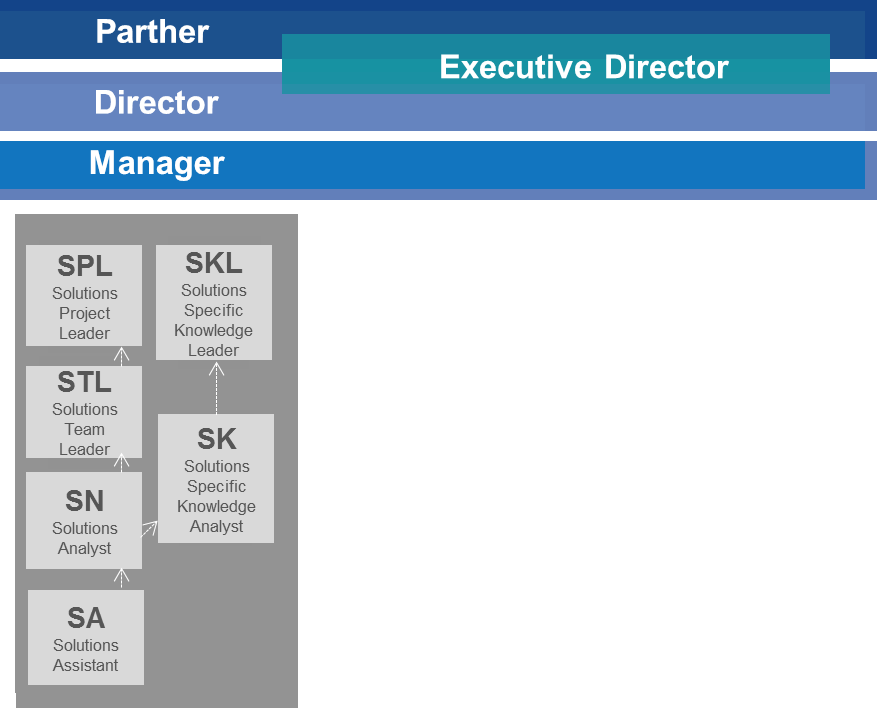
\includegraphics[width=\textwidth]{Cargos-Consultor3}
\caption[Categorías en Tecnología]{Categorías de consultor en la línea operativa
  de Tecnología (\cite{MANUAL}).}
\label{categorias}
\end{figure}

\subsection{Proyecto}
Ejerciendo el cargo de consultor \emph{SA} el estudiante fue asignado al equipo
de arquitectura empresarial \emph{Elara}, el cual está encargado de desarrollar
y mantener las arquitecturas tecnológicas del banco español BBVA.
